\documentclass[final]{beamer}
\mode<presentation>
{
  \usetheme{lspposter}
}
% \usepackage{times} 
\usepackage{amsmath,amssymb}
 \usepackage{textcomp}
% \usepackage{sfmath} % for sans serif math fonts; wget http://dtrx.de/od/tex/sfmath.sty
% \usepackage[english]{babel} 
\usepackage[orientation=portrait,size=a0,scale=1.4,debug]{beamerposter}
\usepackage{booktabs,array}
\usepackage{listings}
\usepackage{xspace}
\usepackage{fp}
\usepackage{ifthen}
% \usepackage[utf8x]{inputenc}
% \usepackage[T1]{fontenc}
% \usepackage{libertine}

\listfiles
\newcommand*{\signstream}{SignStream\texttrademark\xspace}

\graphicspath{{/u/figures/}}

% Display a grid to help align images
%\beamertemplategridbackground[1cm]

\title{\Huge Language Science Press}

\author{Sebastian Nordhoff, FU Berlin}
\institute[Open-Access-Strategie]{Open-Access-Strategie f{\"u}r Berlin} % (optional, but mostly needed)
% {Language Science Press}

\date{13.10.2014}

\begin{document}
\begin{frame}{} 
\vspace{-1cm}
\begin{columns}[t]
  %%%%%%%%%%%%%%%%%%%%%%%%%%%%%%%%%%%%%%%%%%%%%%%%%%%%%%%%%%%%%%%%%%%%%%%%%%%%%%%%%%%%%%%%%%%%%%%%%%%%
  %%%%%%%%%%%%%%%%%%%%%%%%%%%%%%%%%%%%%%%%%%%%%%%%%%%%%%%%%%%%%%%%%%%%%%%%%%%%%%%%%%%%%%%%%%%%%%%%%%%%
  \begin{column}{.45\linewidth}
    

    \setbeamercolor*{block title}{fg=i6colorscheme5,bg=lsp1}
    \begin{block}{Hintergrund}
 \begin{columns}
    \begin{column}{\linewidth}
      \begin{itemize}
      \item Open Access bisher vor allem in den Naturwissenschaften
      \item Andere Publikationskultur in den Geisteswissenschaften \mbox{(mehr Monographien)}
      \item Wie m{\"u}ssen die Modelle der Naturwissenschaften angepasst werden? 
      \end{itemize}
      \end{column}
\end{columns}
    \end{block}    

    \setbeamercolor*{block title}{fg=i6colorscheme5,bg=lsp2}
    \begin{block}{Language Science Press}
 \begin{columns}
    \begin{column}{\linewidth}
      \begin{itemize} 
      \item gef{\"o}rdert von der DFG mit 575.000 EUR f{\"u}r 2 Jahre
      \item ans{\"a}ssig an der FU
      \item 2 Programmierer, 1 Sysadmin, 1 Betriebswirtin, 1 Koordinator
      \end{itemize}
      \end{column}
\end{columns}
    \end{block}
   
    \setbeamercolor*{block title}{fg=i6colorscheme5,bg=lsp3} 
    \begin{block}{Prestige}
      \begin{columns}
	\begin{column}{.48\linewidth}
	  \begin{itemize}
	    \item Spitzenqualit{\"a}t
	    \item Professionelles Design 
	    \item Professionelle Typographie
	    \begin{itemize}
	      \item bessere Zeicheunterst{\"u}tzung als die kommerzielle Konkurrenz
	    \end{itemize}
	  \end{itemize}
	\end{column}
	\begin{column}{.48\linewidth} 
	  
\includegraphics[width=.7\linewidth]{schwaengma.png}
	\end{column}
      \end{columns} 

      \begin{itemize}
	\item Selektivit{\"a}t
	  \begin{itemize}
	    \item keine Dissertationen
	    \item traditioneller Peer Review
	    \item bisher 30\% Ablehnungsquote
	    \item deutlicher Unterschied zu anderen Universit{\"a}tsverlagen
	  \end{itemize}
	\item Renommierte Unterst{\"u}tzer (Harvard, Stanford, Oxford, CNRS) \mbox{aus $>$30 L{\"a}ndern}
	\item Renommierte Reihenherausgeber (u.\,a.\ Luc Steels)
      \end{itemize}
    \end{block}

    \setbeamercolor*{block title}{fg=i6colorscheme5,bg=lsp4}
    \begin{block}{Community}
 \begin{columns}
    \begin{column}{.58\linewidth}
      \begin{itemize}
      \item Reihenbasiert 
      \item Herausgeber organisieren Reihen selbst{\"a}ndig
      \item Begutachtung, Korrektorat, Satz durch Community
      \item Gamificationsystem 
      \end{itemize} 
 \end{column}
    \begin{column}{.38\linewidth}  

\includegraphics[width=.6\textwidth]{barnstar.png}\scalebox{.5}{\tiny \raggedleft   Pic CC-BY Durin, Antonu} 
 \end{column}
 \end{columns}
      \begin{itemize}
      \item international aufgestellte Reihenherausgeber aus 5 Kontinenten
      \item internationale Leser- und Autorenschaft
      \end{itemize}
    \end{block}
 

    \setbeamercolor*{block title}{fg=i6colorscheme5,bg=lsp5}
    \begin{block}{Qualit{\"a}tskontrolle}
      \begin{itemize}
      \item inhaltlich durch Reihenherausgeber
      \item formal (Layout, Satz etc) durch Language Science Press
      \end{itemize} 
    \end{block}

    \setbeamercolor*{block title}{fg=i6colorscheme5,bg=lsp6}
    \begin{block}{Entwicklung}
      \begin{columns}
      \begin{column}{.70\textwidth}
	\begin{itemize}
	  \item Reihen
	    \begin{itemize}
	      \item projiziert: 5 Reihen f{\"u}r 2014
	      \item bereits erreicht: 14 Reihen, 42 Ver{\"o}ffentlichungsanfragen, 
	    \end{itemize} 
	  \item B{\"u}cher
	    \begin{itemize}
	      \item projiziert: 20 B{\"u}cher f{\"u}r 2014
	      \item bereits erreicht: 14 B{\"u}cher
	      \item 42 Ver{\"o}ffentlichungsanfragen bei 30\% Ablehnung $\to$ \mbox{$\sim$28 B{\"u}cher im ersten Jahr}
	    \end{itemize}
	\end{itemize} 
	\end{column}
      \begin{column}{.26\textwidth}
	  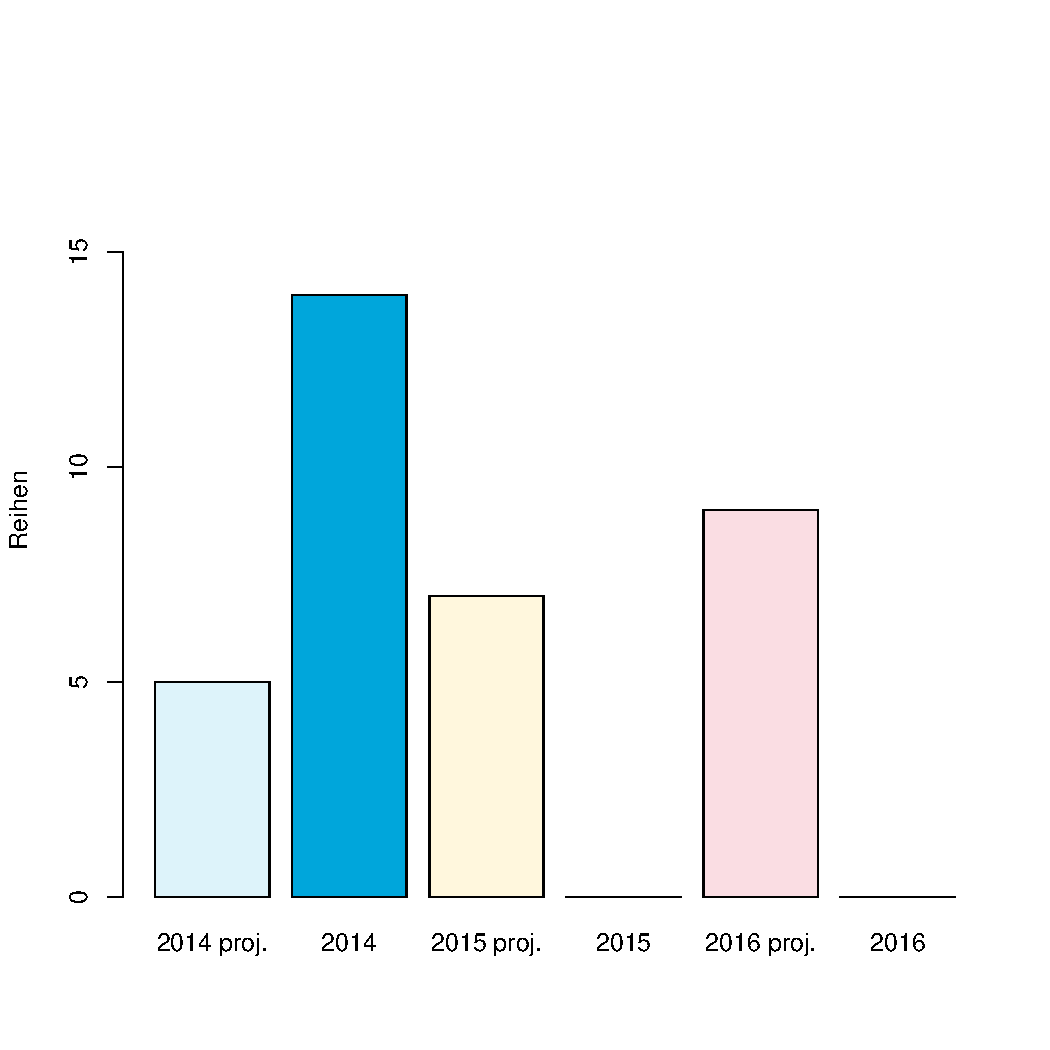
\includegraphics[width=\textwidth]{reihen.pdf} \\
	  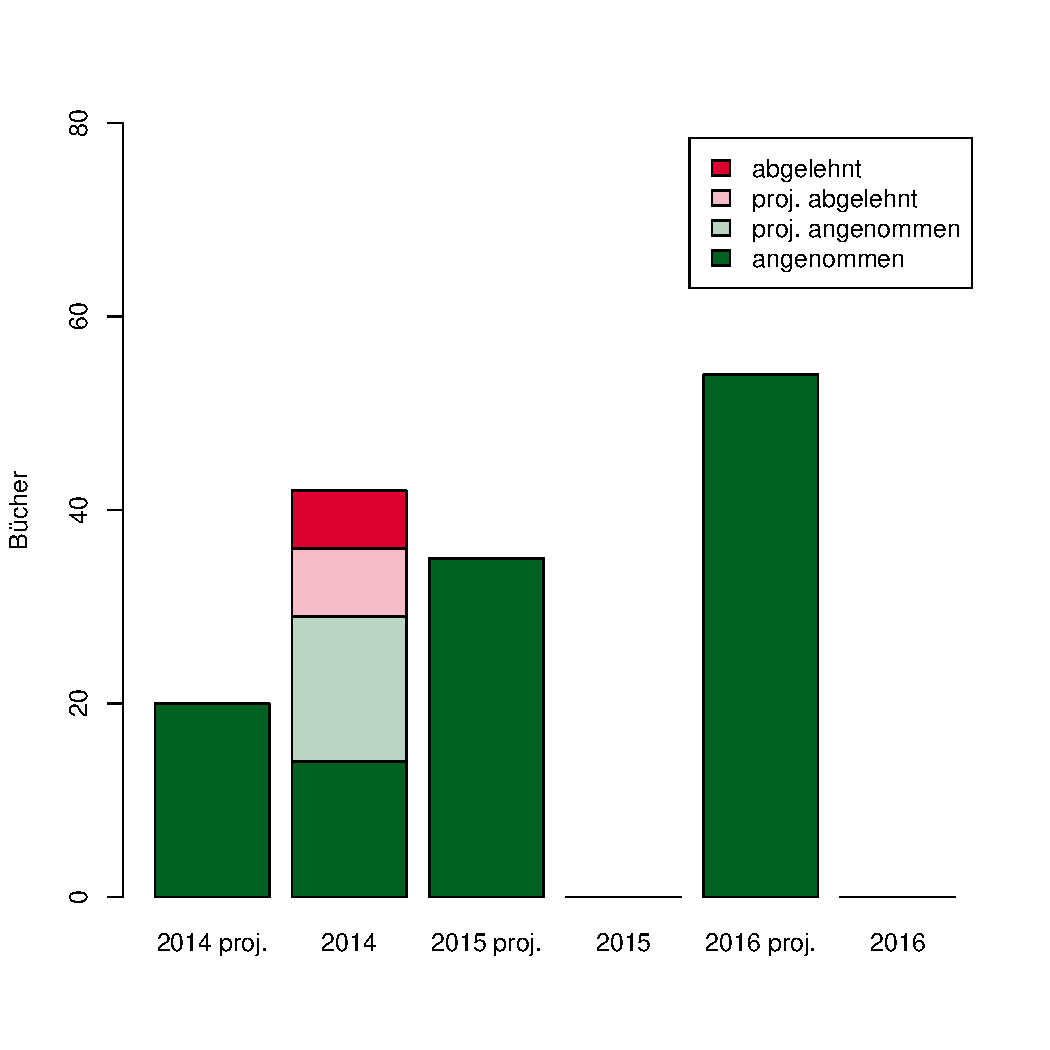
\includegraphics[width=\textwidth]{buecher.pdf}

      
	\end{column}
      \end{columns}
    \end{block}


   
  \end{column}
  %%%%%%%%%%%%%%%%%%%%%%%%%%%%%%%%%%%%%%%%%%%%%%%%%%%%%%%%%%%%%%%%%%%%%%%%%%%%%%%%%%%%%%%%%%%%%%%%%%%%
  %%%%%%%%%%%%%%%%%%%%%%%%%%%%%%%%%%%%%%%%%%%%%%%%%%%%%%%%%%%%%%%%%%%%%%%%%%%%%%%%%%%%%%%%%%%%%%%%%%%%
  \begin{column}{.45\linewidth}
 
    
    \setbeamercolor*{block title}{fg=i6colorscheme5,bg=lsp7}
    \begin{block}{Reihen}
      \begin{columns}
\begin{column}{.48\textwidth}
      \begin{itemize}
      \item African Language Grammars and Dictionaries 
      \item Computational Models of Language Evolution 
      \item Conceptual Foundations of Language Science 
      \item Contemporary African Linguistics
      \item Em­pir­i­cal­ly Ori­ent­ed The­o­ret­i­cal Mor­phol­o­gy and Syn­tax 
      \item Im­ple­ment­ed Gram­mars 
 \item Language Variation 
      \end{itemize}
     \end{column}
\begin{column}{.48\textwidth}
      \begin{itemize}
      \item Lecture Notes in Language Sciences 
      \item Monographs on Comparative Niger-Congo 
      \item Studies in Caribbean Languages 
      \item Studies in Diversity Linguistics 
      \item Studies in Laboratory Phonology 
      \item Topics at the Grammar-Discourse Interface 
      \item Translation and Multilingual Natural Language Processing   
      \end{itemize}
     \end{column}
\end{columns}
      \vskip1ex 
    \end{block}
    
    \setbeamercolor*{block title}{fg=i6colorscheme5,bg=lsp8}
    \begin{block}{B\"{u}cher}
      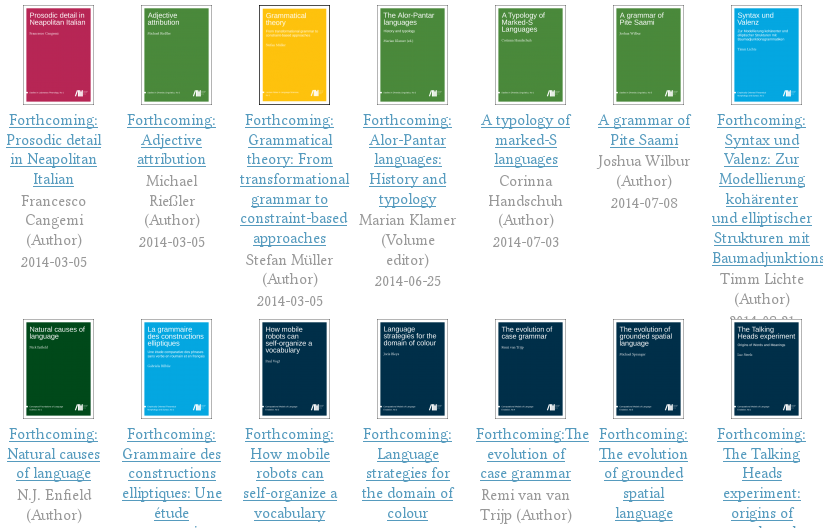
\includegraphics[width=.9\textwidth]{catalog.png}
    \end{block}  
  
    \setbeamercolor*{block title}{fg=i6colorscheme5,bg=lsp9}
    \begin{block}{Vertrieb}
      \begin{columns}
\begin{column}{.48\textwidth}
      \begin{itemize}
      \item Download von Webseite 
      \item Print-on-demand 
      \end{itemize}
\end{column}
\begin{column}{.48\textwidth}
      \begin{itemize}
      \item Google Books 
      \item Amazon
      \end{itemize}
\end{column}
\end{columns}

       
    \end{block}

    \setbeamercolor*{block title}{fg=i6colorscheme5,bg=lsp10}
    \begin{block}{http://www.langsci-press.org}
      \begin{center}
      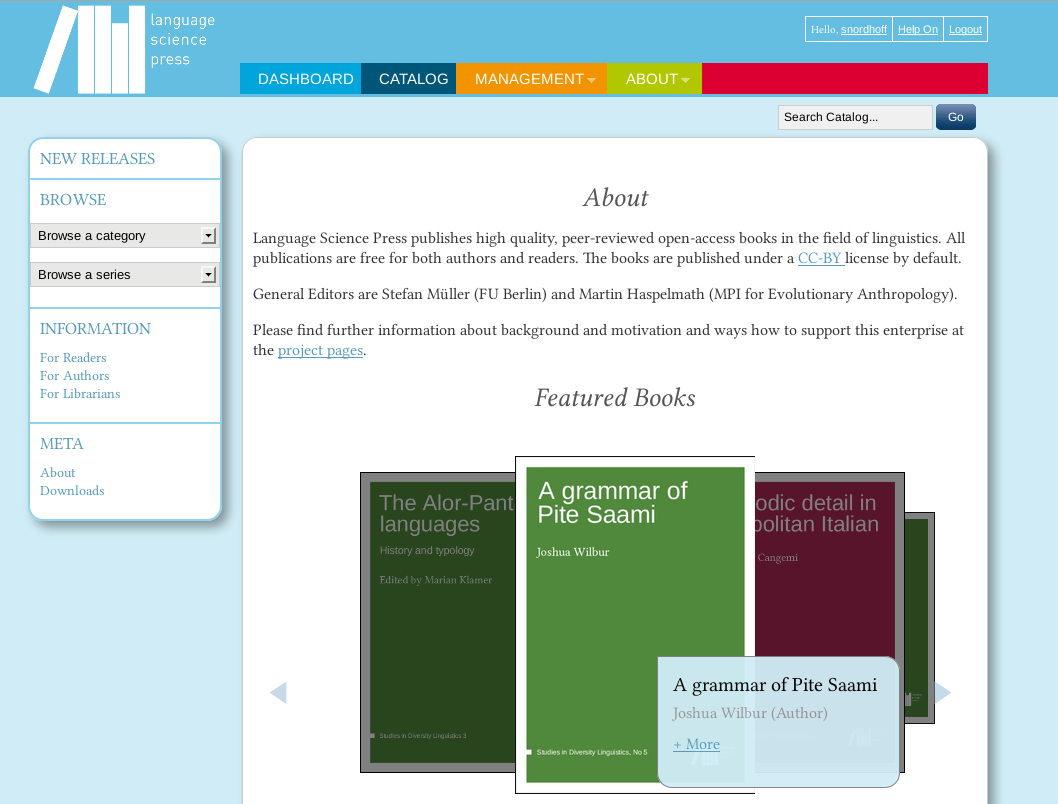
\includegraphics[width=.8\linewidth]{webseite.png}
       
      \end{center} 
    \end{block}

        \setbeamercolor*{block title}{fg=i6colorscheme5,bg=lsp10}
    \begin{block}{Lizenzen}
      \begin{itemize}
       \item Alle Inhalte werden grunds{\"a}tzlich unter CC-BY bereitgestellt
      \end{itemize}
    \end{block}



       
  \end{column}
  %%%%%%%%%%%%%%%%%%%%%%%%%%%%%%%%%%%%%%%%%%%%%%%%%%%%%%%%%%%%%%%%%%%%%%%%%%%%%%%%%%%%%%%%%%%%%%%%%%%%
  %%%%%%%%%%%%%%%%%%%%%%%%%%%%%%%%%%%%%%%%%%%%%%%%%%%%%%%%%%%%%%%%%%%%%%%%%%%%%%%%%%%%%%%%%%%%%%%%%%%%
\end{columns}
\vfill
\end{frame}

\end{document}


%%%%%%%%%%%%%%%%%%%%%%%%%%%%%%%%%%%%%%%%%%%%%%%%%%%%%%%%%%%%%%%%%%%%%%%%%%%%%%%%%%%%%%%%%%%%%%%%%%%%
%%% Local Variables: 
%%% mode: latex
%%% TeX-PDF-mode: t